\documentclass {report}
\usepackage[utf8]{inputenc}
\usepackage{polyglossia}
\usepackage{graphicx}
\usepackage{fancyvrb}

\usepackage{geometry}
 \geometry{
 a4paper,
 total={170mm,257mm},
 left=20mm,
 top=20mm,
 }

\title{Vienkāršu elektrisku shēmu modelēšana}
\author{Dāvis Muižnieks}
\date{2019. gada 13. marts}

\begin{document}

\maketitle
\chapter{Teorētiskā daļa}
\section{Ķēdes aprēķins}

\begin{center}
\small\addtolength{\tabcolsep}{10pt}
\begin{tabular}{|c|c|}
    \hline \multicolumn{2}{|c|}{Tabula:} \\
\hline
R1 & 9Ω\\
\hline
R2 & 8Ω\\
\hline
V1 & 38,7V\\
\hline
$U_{R1}$ & 20,488V\\
\hline
$U_{R2}$ & 18,212V\\
\hline
\end{tabular}
\end{center}
\subsection{Aprēķins}
\textbf{Apliecības numurs: 171RMC100}\\
* $U=V_{1}$ = 38.7V\\
* R$_{1}$ = 9\\
* R$_{2}$ = 8\\
* I = \( \frac{V}{R} \) = \( \frac{38.7}{17}\) = 2.276 A\\
* V$_{R}{1}$ = I*R = 2.276*9 = 20.488 V\\
* V$_{R}{2}$ = I*R = 2.276*8 = 18.212 V\\
* V$_{total}$ = V$_{1}$ + V$_{2}$ = 20.488 + 18.212 = 38.7 V\\

\chapter{Praktiskā daļa}
\section{Darbs ar gEDA programmām}
\subsection{Darbs ar gschem}
\rotatebox{-90}{\includegraphics[width=15cm,height=15cm,keepaspectratio]{pictures/01.ps}}\\
\indent Programmā \textit{gschem} tika sastādīta shēma, atbilstoši veiktajam teorētiskajam aprēķinam (skat. nodaļu Teorētiskā daļa). Katram elementam tika pievienotas atbilstošās vērtības, kuras skatāmas shēmā augstāk. Ar šīs programmas palīdzību tika izveidots ".ps" attēla fails.
\subsection{Darbs ar gnetlist}
\VerbatimInput{text-based/01.net} \\
\hrule
\relax
\indent Ar gnetlist programmu iespējams iegūt netlist failu "*.net", kas satur informāciju par elementu vērtībām, savienojumiem un nosaukumiem no shēmu faila "*.sch"
\subsection{Darbs ar ngspice}
\begin{center}
    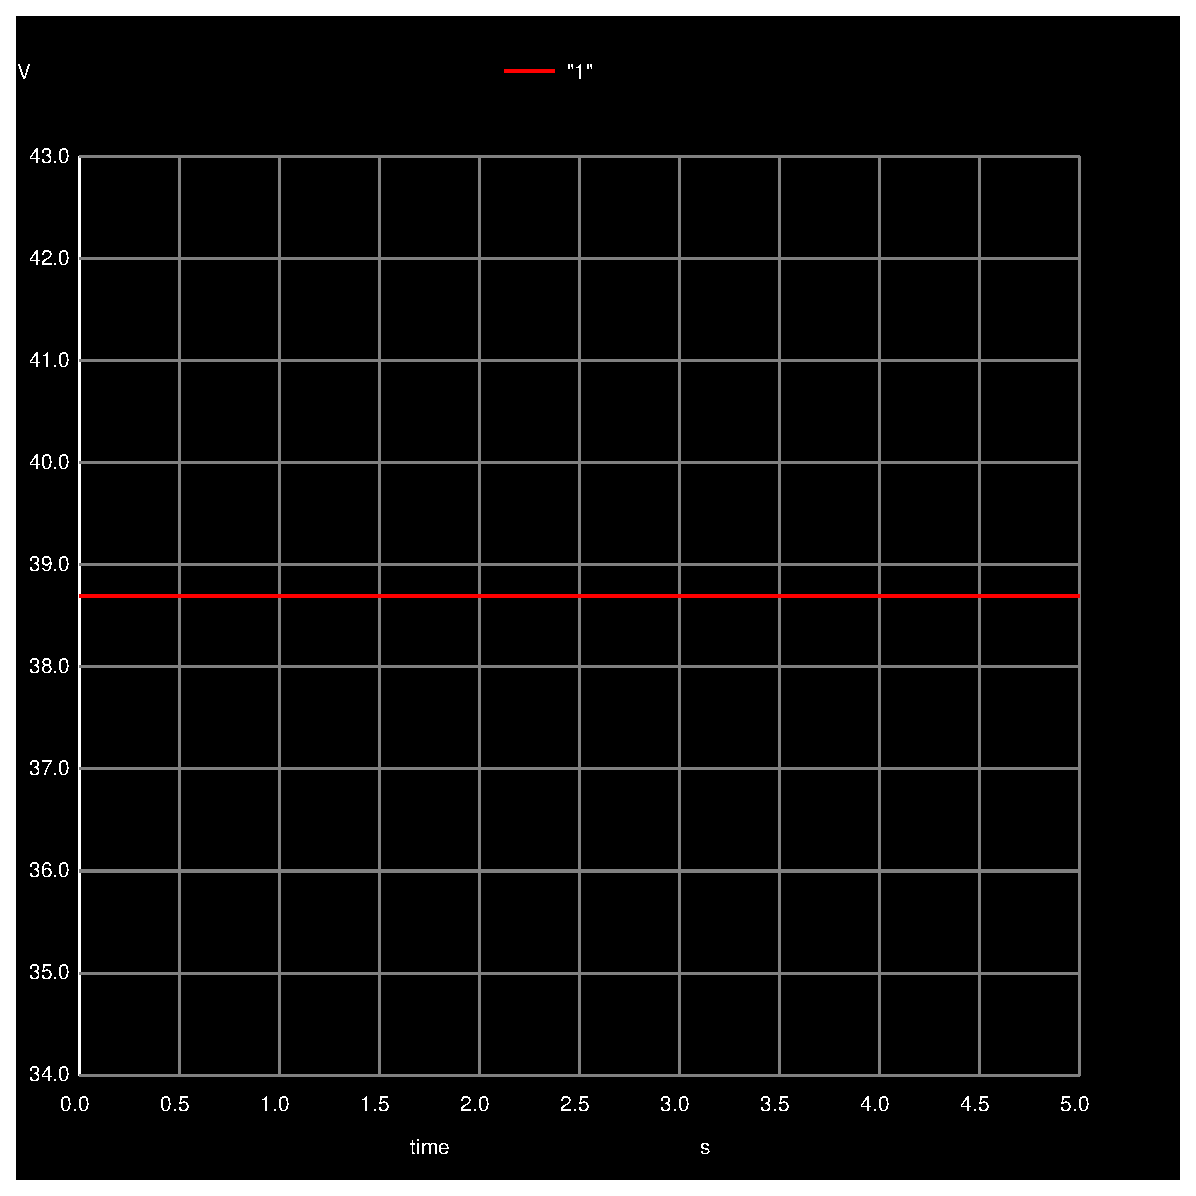
\includegraphics[width=12cm,height=12cm,keepaspectratio]{pictures/011.ps} \textit{1.attēls} \\
    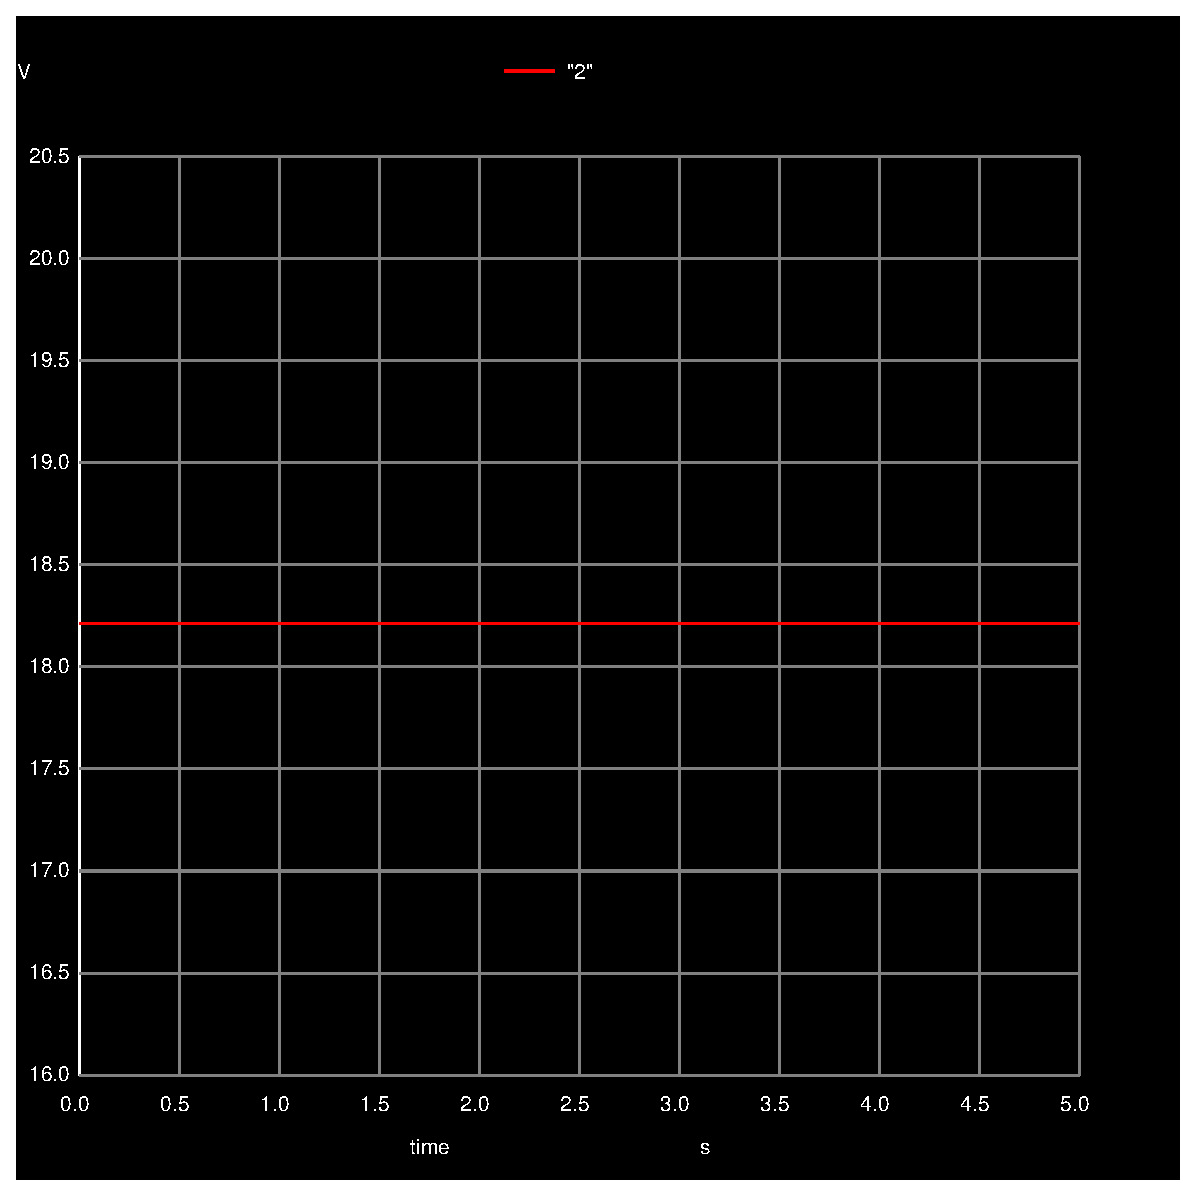
\includegraphics[width=12cm,height=12cm,keepaspectratio]{pictures/012.ps} \textit{2.attēls} \\
\end{center}

\indent Pēc netlist faila pārbaudes ar komandu "cat", to var izmantot simulācijai ar programmu "ngspice". \\
\indent \textbf{1.attēlā} ir attēlots pārejas process (tran) simulācija \textbf{1. signālu savienojumam} no 0 līdz 5 sekundēm ar soli 1 sekunde. \\
\indent \textbf{2.attēlā} ir attēlots pārejas process (tran) simulācija \textbf{2. signālu savienojumam} no 0 līdz 5 sekundēm ar soli 1 sekunde.

\section{Darbs ar QUCS programmām}
\\ QUCS - shēmu simulāciju programma. Ar to iespējams ērti izvēlēties komponentes un veidot savienojumus. Vērtības ir izvēlētas atbilstoši teorētiskajiem aprēķiniem, izņemot R2.
Pricipālā shēma:
\VerbatimInput{schemes/02.sch}
\textbf{Līdzstrāvas simulācijas grafiks:}
\rotatebox{-90}{\includegraphics[width=30cm,height=30cm,keepaspectratio]{pictures/02_scheme.ps}}\\
\indent Izveidotā shēma elementāra līdzstrāvas režīma simulācija ar simulācijas komponenti "Parameter sweep".\\
R2 vietā tiek izmantots mainīgais "x", kas norādīts arī "Parameter sweep" komponentē, kura tiks izmantota sweep simulācijas grafika radīšanai. \\ Veicot simulēšanu, x vērtība (jeb R2) maiņa notiks lineāri, sākot no vērtības 5Ω līdz 50Ω vienpadsmit punktos (sākuma punkts + 10 sekojošie punkti), kuros tiek pārrēķināti visi ķēdes parametri (strāvas un spriegumi) saistrībā ar R2 maiņu.\\
\textbf{Sweep simulācijas līdzstrāvas grafiks un tabula:}
\rotatebox{-90}{\includegraphics[width=60cm,height=30cm,keepaspectratio]{pictures/02.ps}}\\
\indent Iepriekš veiktās simulācijas rezultātā iegūti dati 11 punktos, kurus var izmantot shēmas diagrammu (*.dpl) darba formā. Izvēloties Dekarta koordinātu sistēmas diagrammu komponenti un punktu "izeja", iegūstam grafiku, kas rāda funkcionālu sakarību starp mainīgo R2 vērtību un spriegumu uz tā - UR2. \indent UZ darba formas atrodas arī tabula, kurā attēlota strāvu "V1.I" (plūst caur sprieguma avotu V1) un el. ķēdes punkta "Izeja" attiecība.

\end{document}
